% Source: AESP_466_ClassWork/Supplements/Notes/latex/6.6/6.6.tex

\documentclass[border=4pt]{standalone}
\usepackage{amsmath,amssymb,amsthm}
\usepackage{graphicx}
\usepackage{tikz}
\usepackage{xcolor}
\usetikzlibrary{arrows.meta,calc,positioning,decorations.markings,patterns,shapes.geometric,angles,quotes}

\definecolor{Garnet}{HTML}{73000A}
\definecolor{USC_Rose}{HTML}{CC2E40}
\definecolor{USC_Blue}{HTML}{466A9F}
\definecolor{USC_Slate}{HTML}{1F414D}
\definecolor{USC_Olive}{HTML}{65780B}
\definecolor{USC_Lime}{HTML}{CED318}
\definecolor{USC_Gold}{HTML}{A49137}
\definecolor{USC_Black90}{HTML}{565556}
\definecolor{USC_Black10}{HTML}{ECECEC}

\newcommand{\vect}[1]{\mathbf{#1}}
\newcommand{\mat}[1]{\mathbf{#1}}
\newcommand{\uvec}[1]{\hat{\mathbf{#1}}}
\newcommand{\transpose}{^{\mkern-1.5mu\mathsf{T}}}
\newcommand{\inv}{^{-1}}
\newcommand{\deriv}[2]{\frac{d #1}{d #2}}
\newcommand{\pderiv}[2]{\frac{\partial #1}{\partial #2}}

\begin{document}
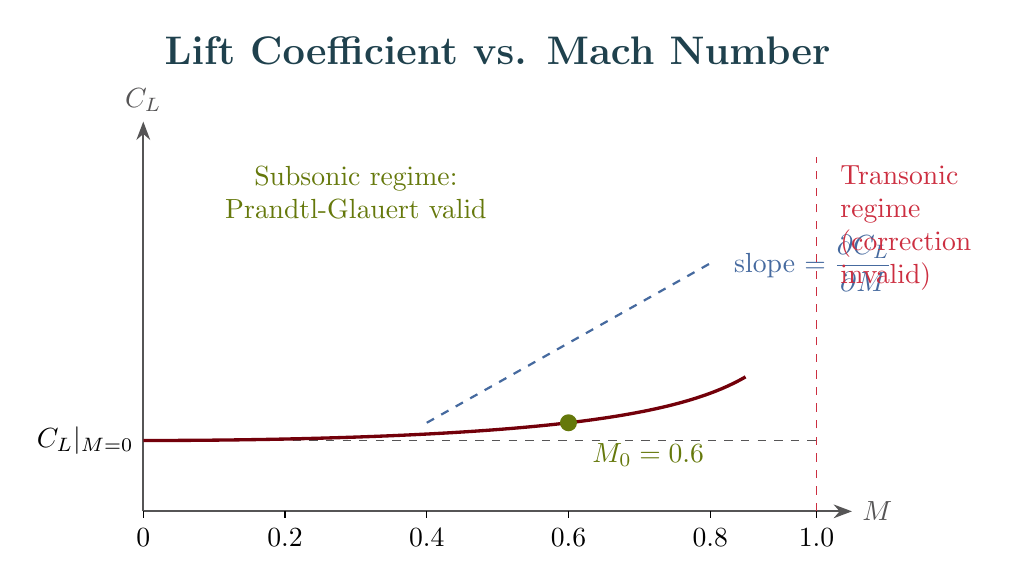
\begin{tikzpicture}[>=Stealth, scale=0.9]
    % Title
    \node[font=\Large\bfseries, USC_Slate] at (5,6.5) {Lift Coefficient vs. Mach Number};

    % Axes
    \draw[->, thick, USC_Black90] (0,0) -- (10,0) node[right] {$M$};
    \draw[->, thick, USC_Black90] (0,0) -- (0,5.5) node[above] {$C_L$};

    % Mach number labels
    \foreach \x/\label in {0/0, 2/0.2, 4/0.4, 6/0.6, 8/0.8, 9.5/1.0} {
        \draw (\x,0) -- (\x,-0.1);
        \node[below] at (\x,-0.1) {\label};
    }

    % CL axis labels
    \node[left] at (0,1) {$C_L|_{M=0}$};
    \draw[dashed, USC_Black90] (0,1) -- (9.5,1);

    % Prandtl-Glauert curve (1/sqrt(1-M^2) scaled)
    \draw[very thick, Garnet, domain=0:8.5, samples=100]
        plot (\x, {1/sqrt(1-(\x/10)^2)});

    % Tangent line at M=0.6 showing derivative
    \draw[thick, USC_Blue, dashed] (4,1.25) -- (8,3.5);
    \node[USC_Blue, right] at (8.2,3.5) {slope $= \dfrac{\partial C_L}{\partial M}$};

    % Point at M=0.6
    \fill[USC_Olive] (6,1.25) circle (0.12);
    \node[USC_Olive, below right] at (6.2,1.1) {$M_0 = 0.6$};

    % Annotation for asymptote
    \draw[dashed, USC_Rose] (9.5,0) -- (9.5,5);
    \node[USC_Rose, right, align=left] at (9.7,4) {Transonic\\regime\\(correction\\invalid)};

    % Region labels
    \node[USC_Olive, align=center] at (3,4.5) {Subsonic regime:\\Prandtl-Glauert valid};

\end{tikzpicture}
\end{document}
